\chapter{Simulation and Results}
\label{chap:5_Simulation_And_Results}
        
    % Grammarlly: 95/100
    In this chapter, we present simulation scenarios for qualitative and quantitative evaluation of our system, as well as the experimental results. The simulations cover different encounter scenarios between two vessels, one using our path planning method and other without any COLREGS-compliant method. For qualitative evaluation, we analyzed avoidance success and the behavior of our system when exposed to different environmental conditions. For quantitative evaluation, we analyzed the time for computation of our path planning method and the minimum distance kept between our COLREGS-compliant vessel and the encountering vessel during the simulation.

    \section{Simulations Characterization}

    % Grammarlly: 100/100
    We run our simulations on USV\_sim\footnote{https://github.com/disaster-robotics-proalertas/usv\_sim\_lsa}~\cite{Paravisi2018Toward} simulator using the platform described in Table \ref{tab:simulation_platform_description}. 
    We developed 12 scenarios for evaluation the system focusing on comparison with simulations presented in reference studies, \ie{} Agrawal \etal{} ~\cite{Agrawal2015COLREGS} and Huang \etal{} ~\cite{Huang2019Generalized}. We chose both studies for their quality (\ie{} h-index > 50) and similarity with our work. Agrawal \etal{} present our problem-solving inspiration but unfortunately, they do not present too much information about their system evaluation, so we based our tests and system evaluation on Huang \etal{} as they explicitly present their simulation scenarios characterization, results, and simulate a \ac{USV} similar to ours in respect to the dimensions.
    
    \taburowcolors[1] 1{tableLineOne .. tableLineTwo}
    \tabulinesep = ^3mm_2mm
    \everyrow{\tabucline[.4mm  white]{}}

    \begin{table}[H]
        \caption{Simulation Platform Description}
        \centering
            \begin{tabu} to \textwidth { >{\bfseries}X[c, 0] X[c, 3]}
            \tableHeaderStyle
            Component & Specification \\
            Computer & Desktop Dell XPS 8700 \\
            Processor & Intel® Core™ i7-4770 CPU @ 3.40GHz × 8 \\
            Memory & \begin{tabular}[c]{@{}l@{}}Teikon PC3-12800u DDR3 1600 MHz 2GB x 2\\ Teikon PC3-12800u DDR3 1600 MHz 4GB x 2\end{tabular} \\
            Operating System & Ubuntu 16.04.6 LTS \\
            ROS Version & ROS Kinetic
            \end{tabu}  
        \label{tab:simulation_platform_description}
    \end{table}
    
    % Grammarlly: 100/100
    In our simulations, we use a differential boat - shown in Figure \ref{fig:diffboat} - with two thrusters, which enables it to rotate over its axis. This boat is modeled according to specifications of the Lutra Prop boat, acquired from Platypus ~\cite{PlatypusLLC}. Beyond the specifications shown in Table \ref{tab:diffboat_specs}, the Lutra boat we use in our simulation has a laser rangefinder for environment scanning in its bow. We set the rangefinder to be capable of detecting objects within 25 meters in a range of 360°.
    
    % \taburowcolors[1] 1{tableLineOne .. tableLineTwo}
    % \tabulinesep = ^3mm_2mm
    % \everyrow{\tabucline[.4mm  white]{}}
    % \begin{table}
    %     \caption{Lutra Prop parameters}
    %     \centering
    %         \begin{tabu} to 0.45\textwidth { >{\bfseries}X[c, 2] X[c, 2]}
    %         \tableHeaderStyle
    %         Parameter       & Value       \\
    %         Length          & 106 cm      \\
    %         Width           & 48 cm       \\
    %         Height          & 15 cm       \\
    %         % Hull Volume     & ~0.02 $m^3$ \\
    %         Weight          & 9.7 Kg      \\
    %         % Extra Payload   & 3 Kg        \\
    %         % Thruster Force  & 22.54 N     \\
    %         % Linear drag     & 11.33       \\
    %         Maximum speed   & 1.41 m/s    \\
    %         \end{tabu}  
    %     \label{tab:simulation_platform_description}
    % \end{table}
    
    \begin{minipage}{\textwidth}
        \begin{minipage}[b]{0.35\textwidth}
        \centering
        \begin{figure}[H]
            \centering
            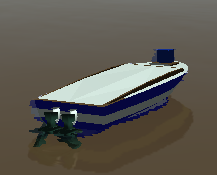
\includegraphics[scale=0.75]{figs/Chap5/diffboat.png}
            % \caption{Simulated version of Lutra Prop boat}
            % \label{fig:diffboat}
        \end{figure}
        \captionof{figure}{Simulated version of Lutra Prop boat}
        \label{fig:diffboat}
        \end{minipage}
    %   \hfill
        \begin{minipage}[b]{0.5\textwidth}
        \centering
            \begin{tabular}{cc}
                \toprule
                    \textbf{Parameter}       & \textbf{Value}       \\
                \midrule
                    Length          & 106 cm      \\
                    Width           & 48 cm       \\
                    Height          & 15 cm       \\
                    Weight          & 9.7 Kg      \\
                    Maximum speed   & 1.41 m/s    \\ 
                \bottomrule
            \end{tabular}
        \captionof{table}{Lutra Prop parameters}
        \label{tab:diffboat_specs}
        \end{minipage}
    \end{minipage}
    
    \vskip 1cm

    % Grammarlly: 100/100
    We assembled the scenarios in a simulated version of the Dilúvio stream. The Dilúvio stream is a potential location for real-world trials of our system since it is near our laboratory, so we evaluate the behavior of our system on a simulated version of it. In Figure \ref{fig:simulation_diluvio_googleLocation2_roundedArea} we show with a red box the specific location we simulated in our experiments\footnote{Google maps location: (-30.047258°, -51.232660°), Av. Edvaldo Pereira Paiva, 1970 - Praia de Belas - Porto Alegre - RS - Brazil} and its simulated version.
    % We assembled 4 encounters between two vessels in the region marked with the red box.
     %AMA mencionar brevemente como esse cenario foi montado (foto area, resolucao de tanto, etc). O Marcelo tem essa descricao.
    % Este cenário foi criado pelos mantedores do USV\_sim. Ele foi construído unindo informação geográfica de localização e relevo com informação de geometria e edificações 3D. Este cenário simula uma área real de 1340mx555m.
     
    \begin{figure}
    \centering
        \begin{subfigure}[b]{0.48\textwidth}
            \centering
            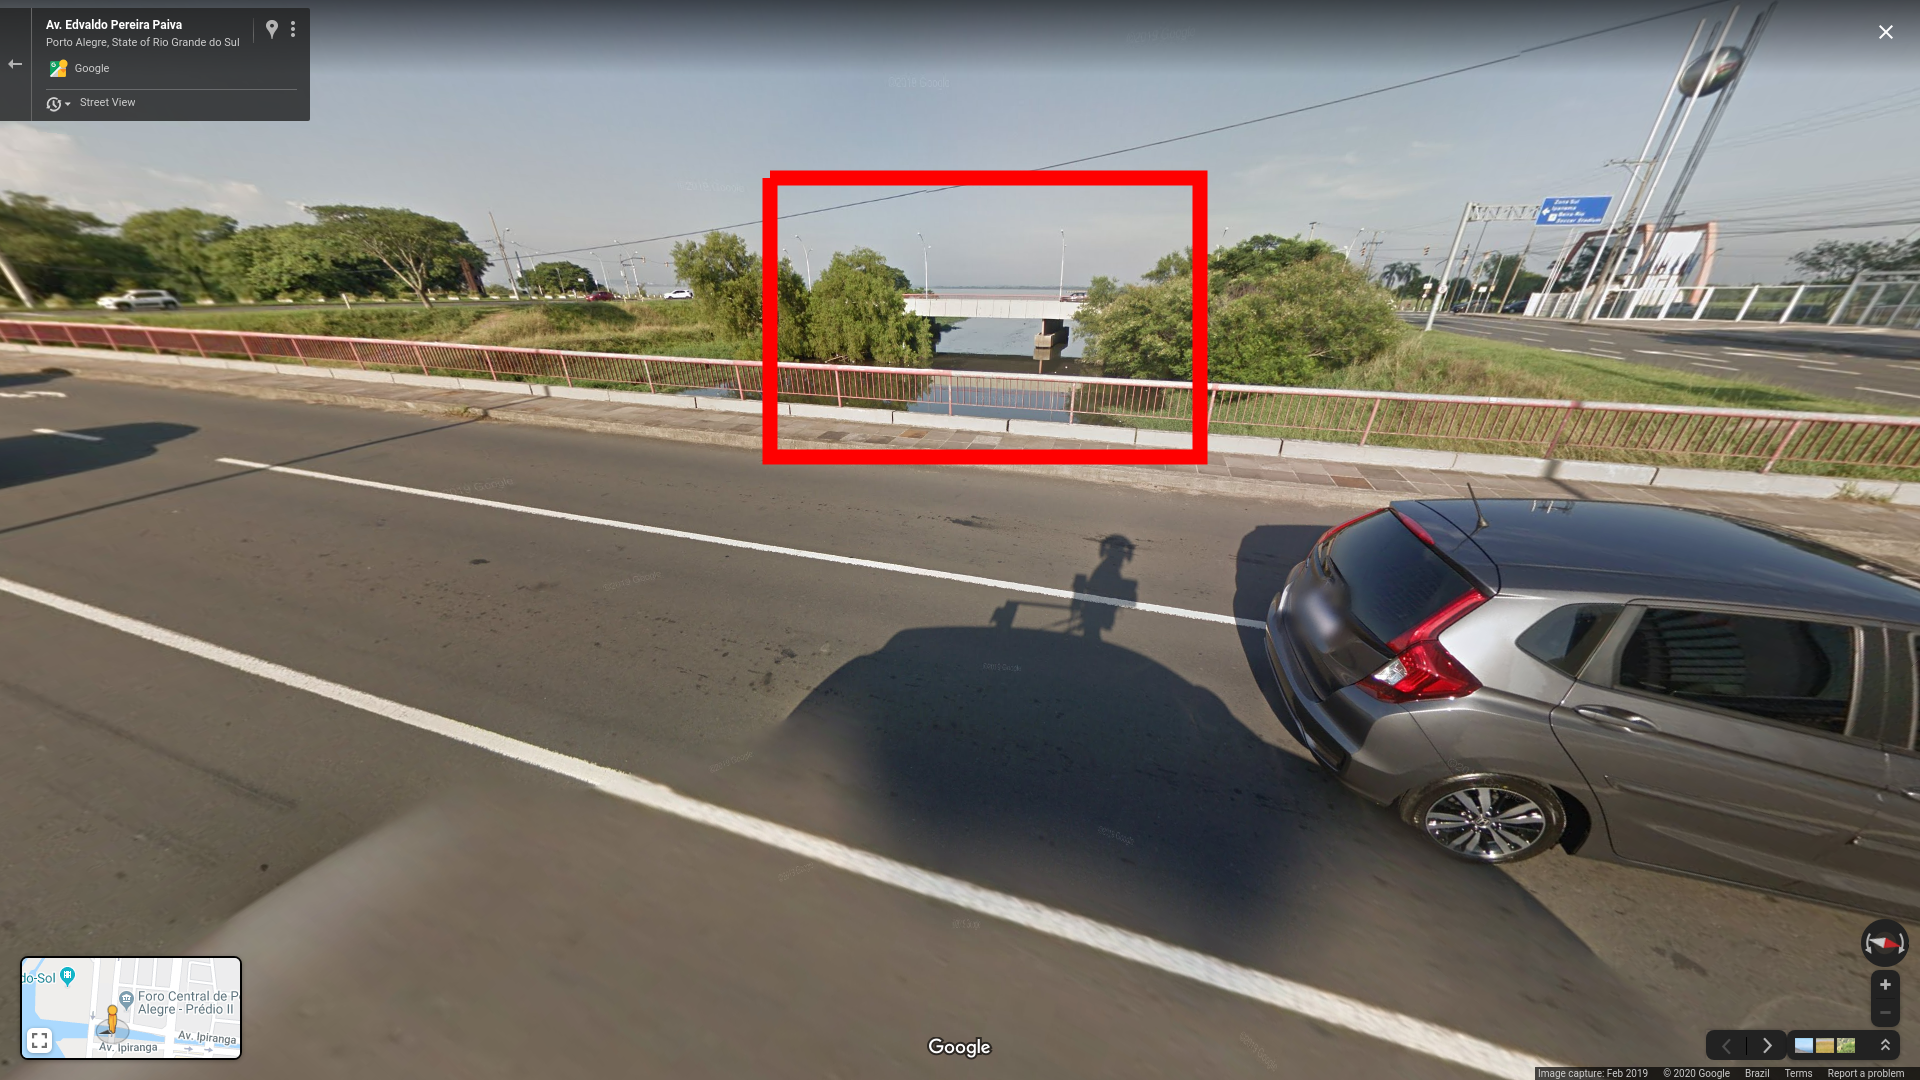
\includegraphics[scale=0.12]{figs/Chap5/simulation_diluvio_googleLocation2_1_roundedArea.png}
            \caption{Real World Location}
            \label{fig:simulation_diluvio_googleLocation2_1_roundedArea}
        \end{subfigure}
        \hfill
        \begin{subfigure}[b]{0.48\textwidth}
            \centering
            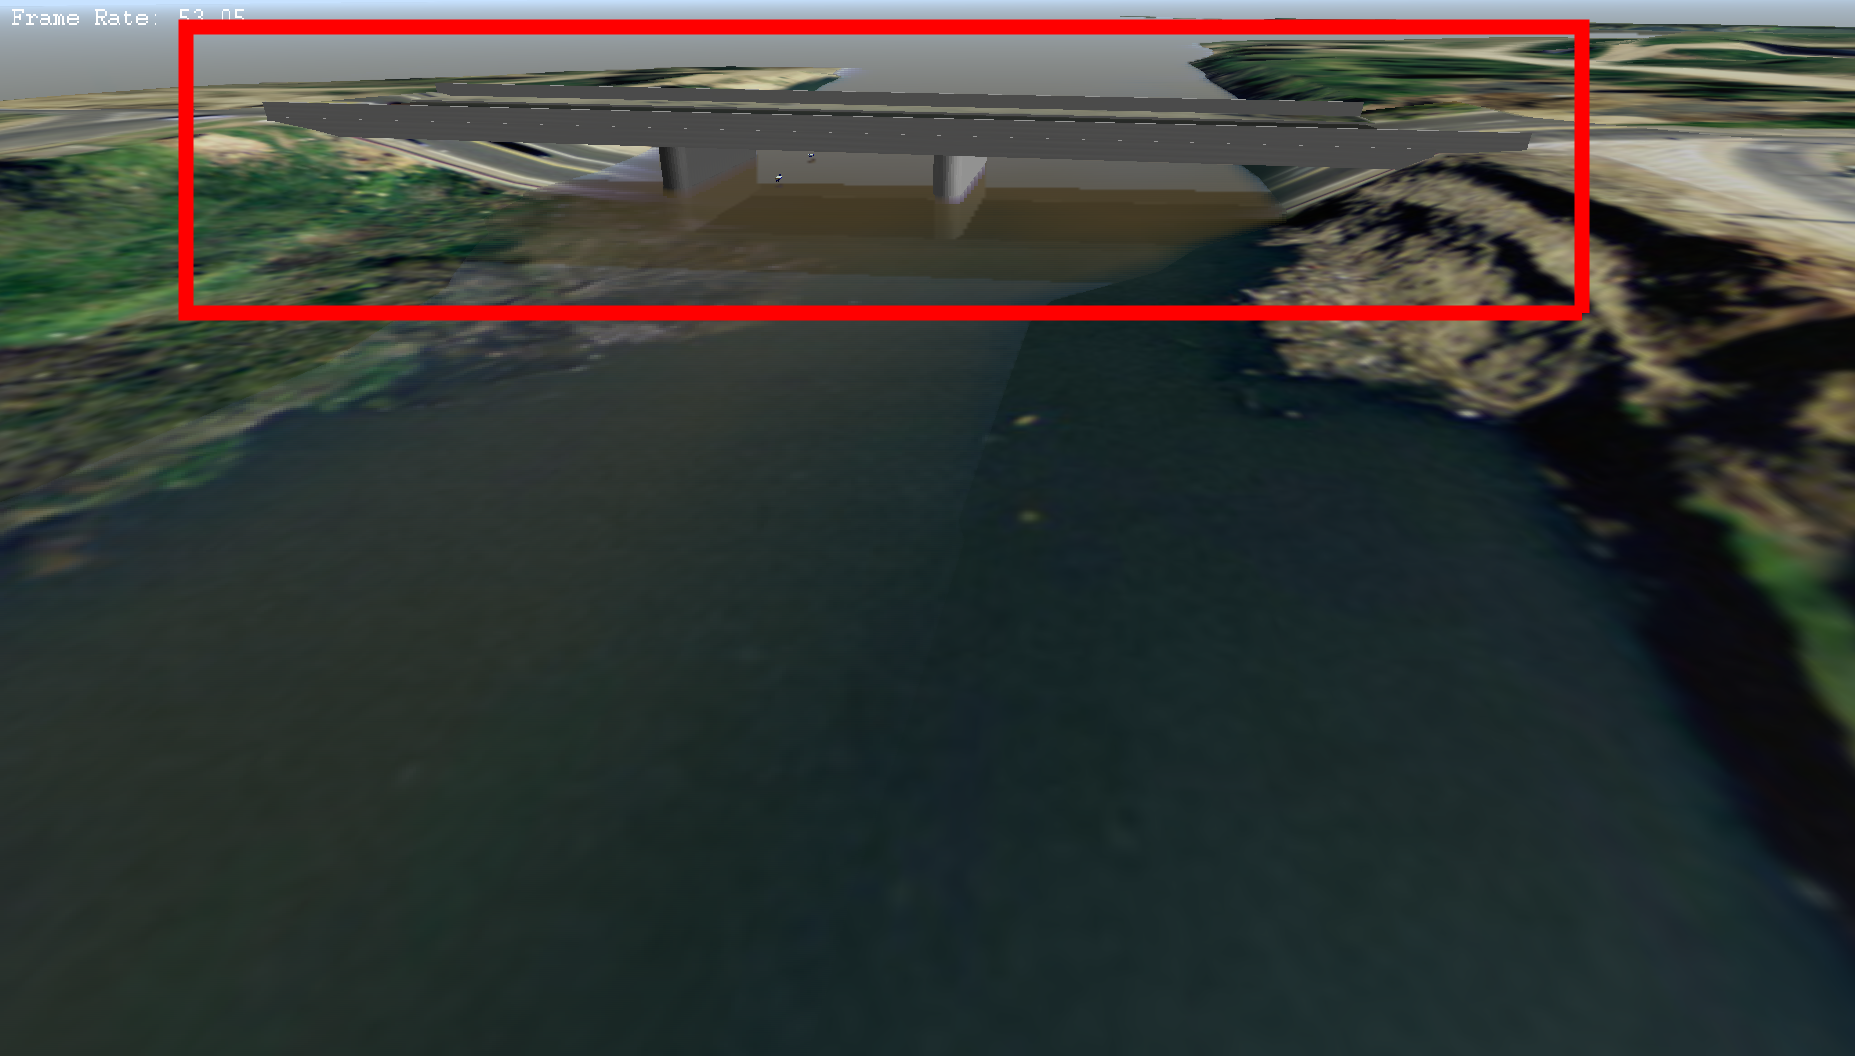
\includegraphics[scale=0.122]{figs/Chap5/simulation_diluvio_googleLocation2_2_roundedArea.png}
            \caption{Simulated version of Real World Location }
            \label{fig:simulation_diluvio_googleLocation2_2_roundedArea}
        \end{subfigure}
    
    \caption{Real world region and its simulated version}
    \label{fig:simulation_diluvio_googleLocation2_roundedArea}
    \end{figure}
     
    % V1.0:  
    % As done by several authors, \eg{} Larson \etal{}~\cite{Larson2006Autonomous}, Naeem \etal{}~\cite{Naeem2012COLREGS}, Campbell \etal{}~\cite{Campbell2013Automatic}, Naus~\cite{Naus2013Idea}, \etc{}, we evaluated 4 main encounter scenarios between two vessels, head-on, crossing from the right, crossing from the left, and overtaking. 
    % V2.0:  
    % Grammarlly: 100/100
    As done by several authors (\eg{} Larson \etal{}~\cite{Larson2006Autonomous}, Naeem \etal{}~\cite{Naeem2012COLREGS}, Campbell \etal{}~\cite{Campbell2013Automatic}, Naus~\cite{Naus2013Idea}), regarding evaluate the \ac{COLREGS}-compliance of our system, we assembled 4 main encounter scenarios between two vessels, head-on, crossing from the right, crossing from the left, and overtaking. One of the vessels own our \ac{COLREGS}-compliant system (forthworth referred as \acl{OV}) the other vessel (forthworth referred as \acl{AV}) don't have any \ac{COLREGS} compliance knowledge. The starting configuration of each vessel in each scenario is described in Tables \ref{tab:simulation_scenarios_configuration_own_vessel} and \ref{tab:simulation_scenarios_configuration_encountering_vessel}. Both head-on and overtaking scenarios, were assembled right below the bridge shown in Figure \ref{fig:simulation_diluvio_googleLocation2_roundedArea}, while the crossing scenarios were assembled far the bridge, simply due to the need of more space between the start positions.

%   \begin{figure}
%         \centering
%         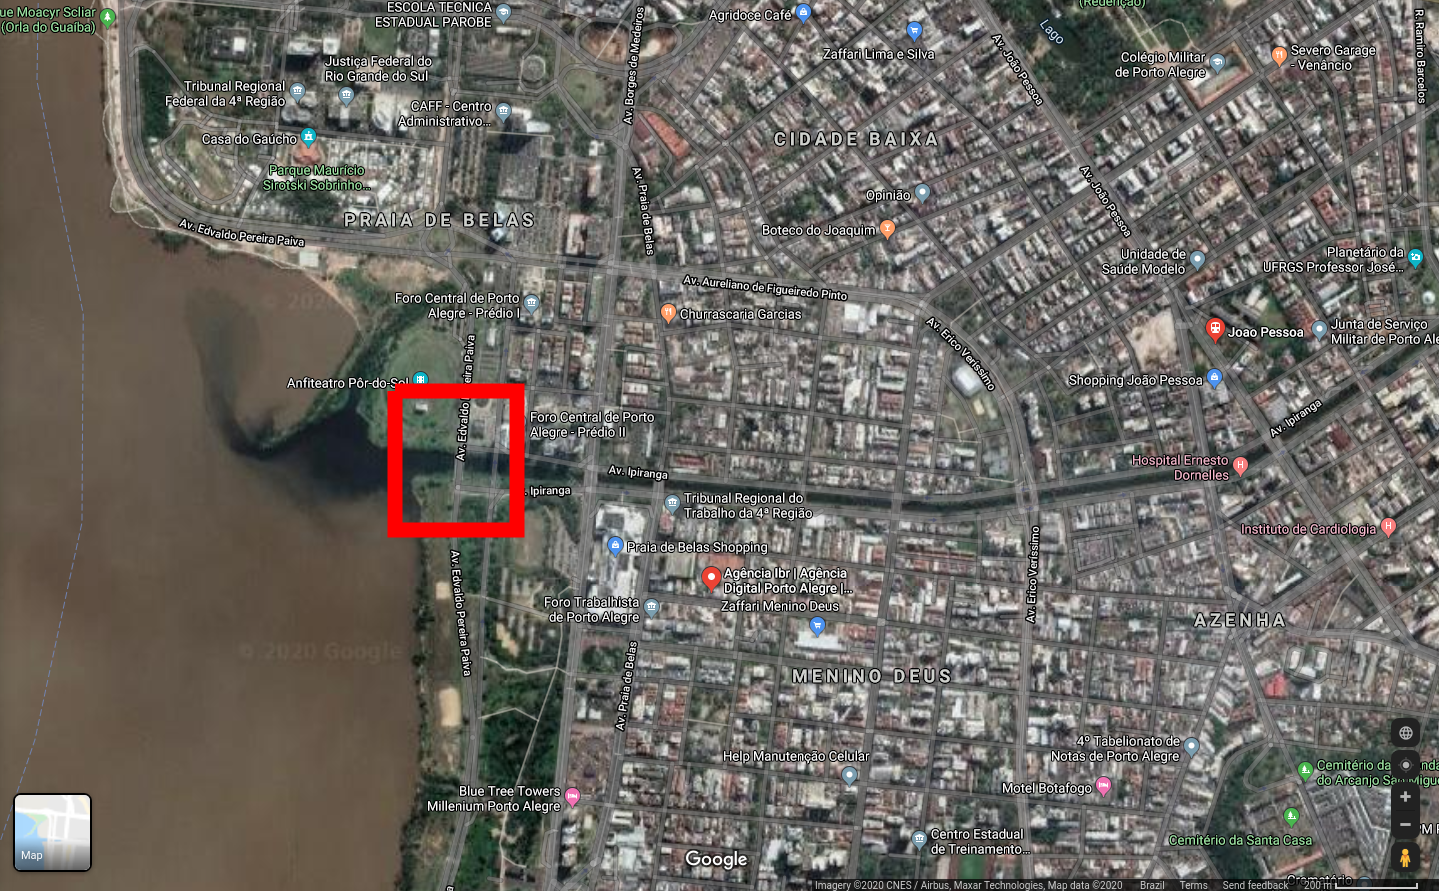
\includegraphics[scale=0.32]{figs/Chap5/simulation_diluvio_googleLocation_roundedArea.png}
%         \caption{Real-world location of the area we choose for evaluation of our system.}
%         \label{fig:simulation_diluvio_googleLocation_roundedArea}
%     \end{figure}
    % \todo{cite some characteristics of the region}
    
    \begin{figure}[H]
    \centering
    
        \begin{subfigure}[b]{0.495\textwidth}
            \centering
            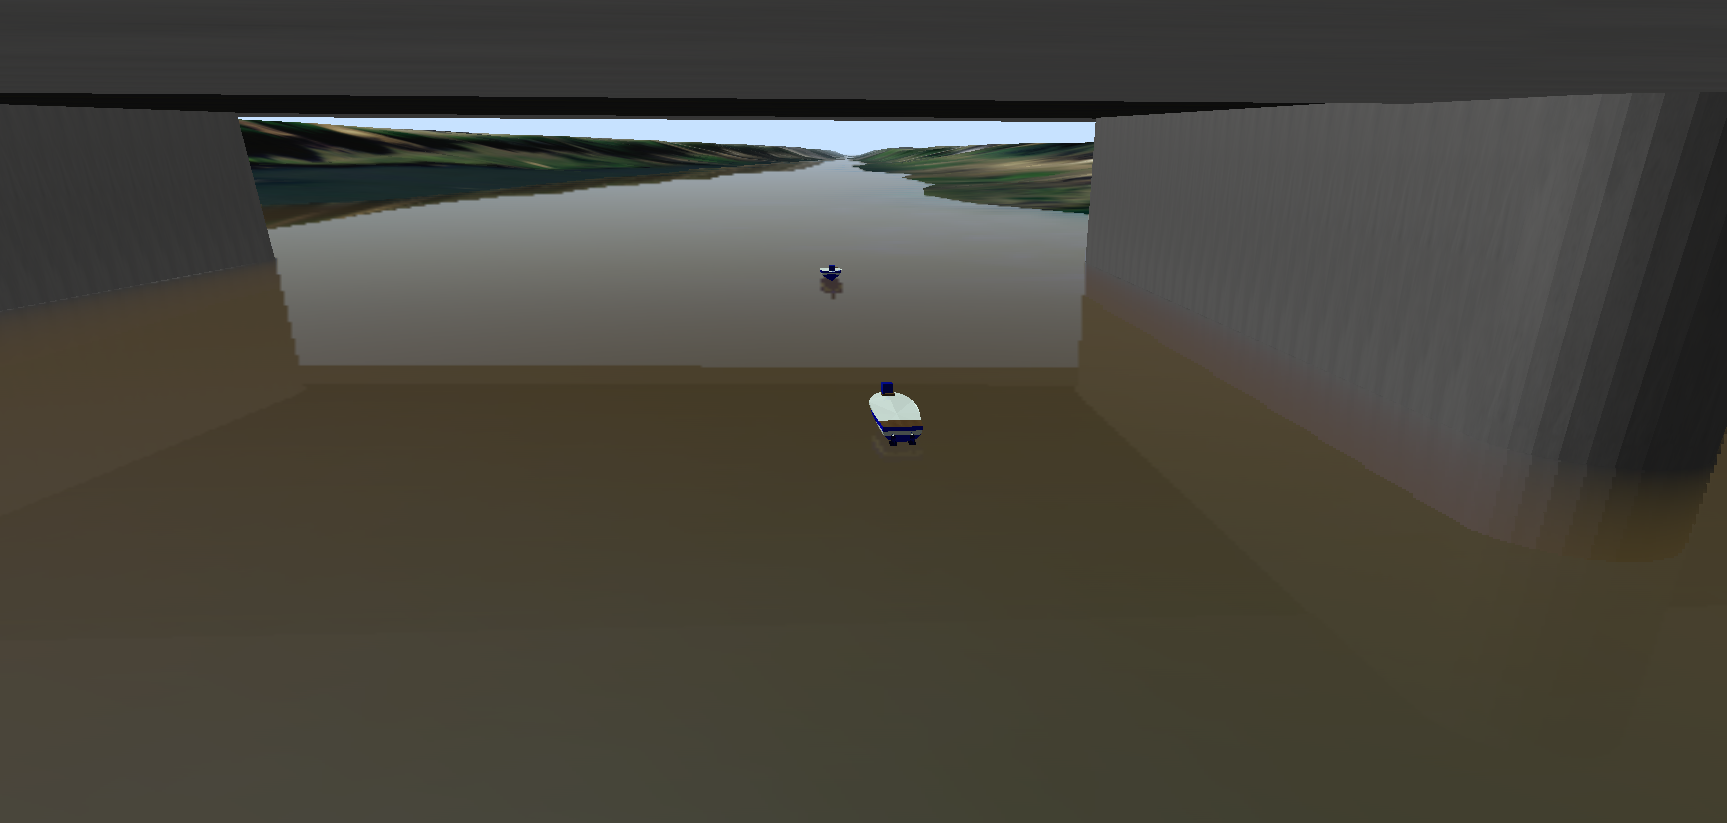
\includegraphics[width=\textwidth]{figs/Chap5/simulation_uwsim_headon_starting_pos.png}
            \caption{Head-on Encounter.}
            \label{fig:simulation_uwsim_headon_starting_pos}
        \end{subfigure}
        \begin{subfigure}[b]{0.495\textwidth}
            \centering
            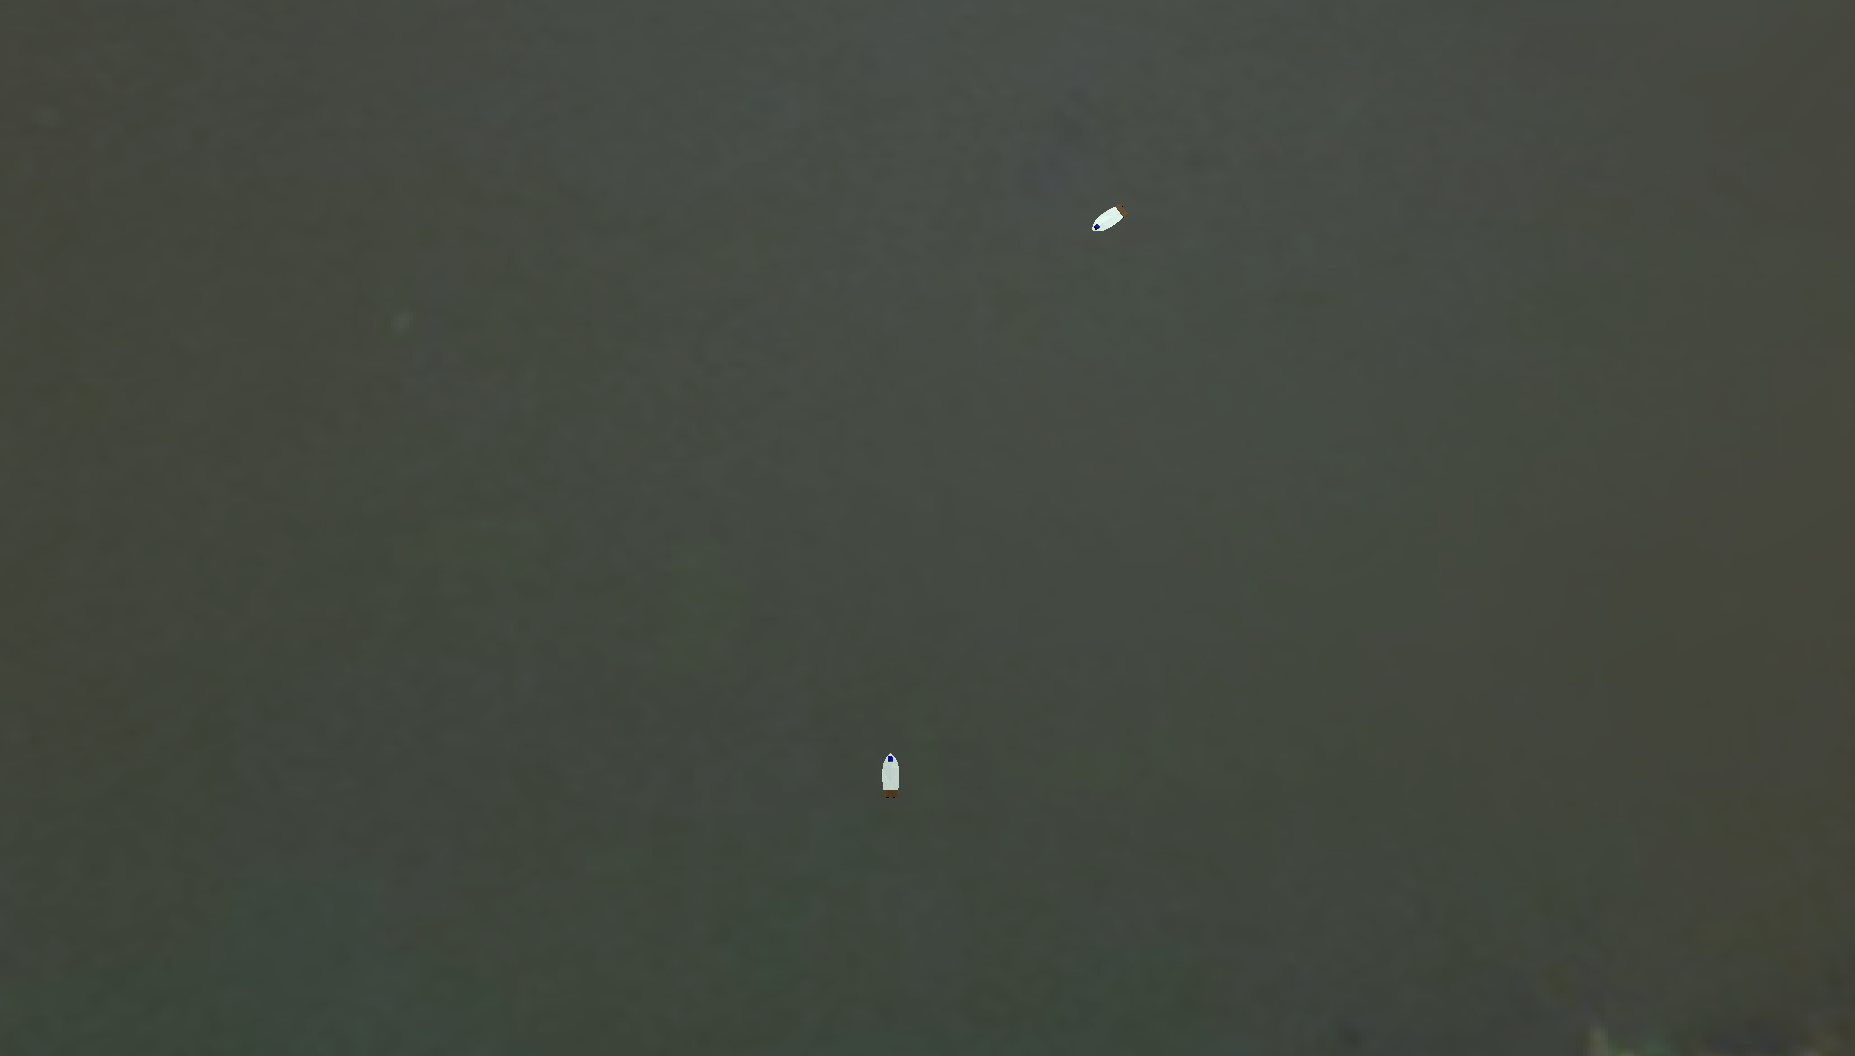
\includegraphics[width=\textwidth]{figs/Chap5/simulation_uwsim_crossingright_starting_pos.png}
            \caption{Crossing from Right}
            \label{fig:simulation_uwsim_crossingright_starting_pos}
        \end{subfigure}
        
        \begin{subfigure}[b]{0.495\textwidth}
            \centering
            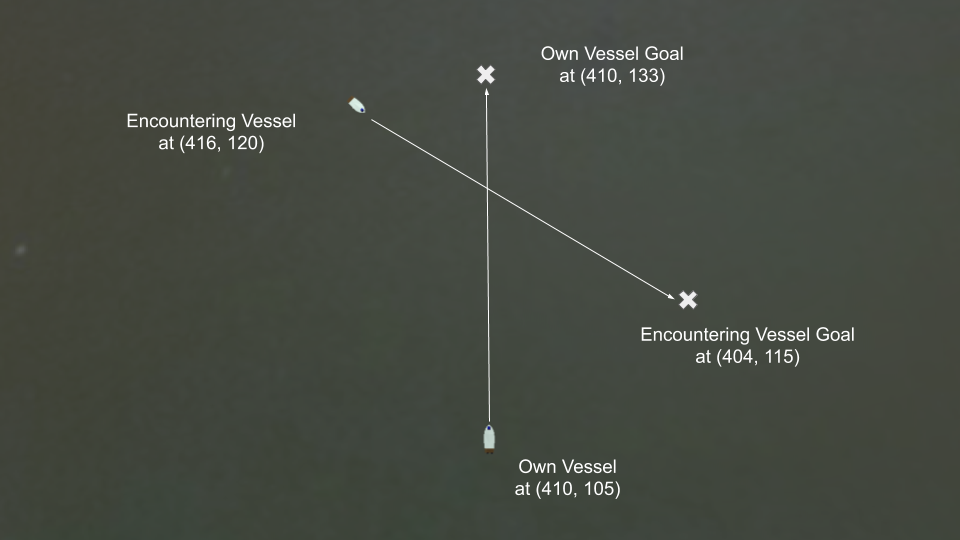
\includegraphics[width=\textwidth]{figs/Chap5/simulation_uwsim_crossingleft_starting_pos.png}
            \caption{Crossing from Left}
            \label{fig:simulation_uwsim_crossingleft_starting_pos}
        \end{subfigure}
        \begin{subfigure}[b]{0.495\textwidth}
            \centering
            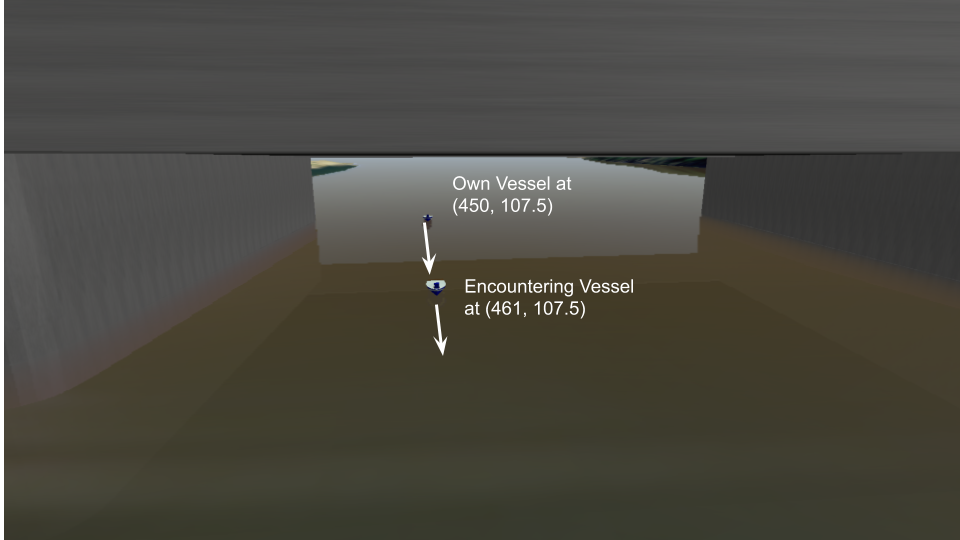
\includegraphics[width=\textwidth]{figs/Chap5/simulation_uwsim_overtake_starting_pos.png}
            \caption{Overtaking}
            \label{fig:simulation_uwsim_overtake_starting_pos}
        \end{subfigure}
    
    \caption{Encounter scenarios for evaluation. Scenarios adapted from ~\cite{Huang2019Generalized}.}
    \label{fig:simulation_uwsim_encounters}
    \end{figure}

%AMA o que siginifica OV na tab 5.3 ?
%DJ: Done

    \begin{center}
        \savebox{\mytablebox}{\begin{tabular}{cccc}
        
        \toprule[3pt]
        \multicolumn{4}{c}{\textbf{\acf{OV}}} \\
        % \multicolumn{3}{c}{\textbf{\ac{OV}}} \\
        \midrule
        \textbf{Encounter Type} & \textbf{Initial Pose (m, m, º)} & \textbf{Target Position} &  \textbf{Max. Speed (m/s)}\\
        \midrule
        Head On &  (450, 107.5, 0)  &   (480, 107.5)  &  0.47 \\
        Crossing Right &  (410, 105, 90)  &  (410, 133)  &  0.43  \\
        Crossing Left &  (410, 105, 90)  & (410, 133)   &  0.33  \\
        Overtaking &  (450, 107.5, 0)  &  (600, 107.5) &  0.5 \\
        \bottomrule
        
        \end{tabular}}
        \settowidth{\mytablewidth}{\usebox{\mytablebox}}
        \begin{minipage}{\mytablewidth}
        \captionof{table}{Encounter Scenarios Configuration and maximun achieved speed - \ac{OV}}
        \label{tab:simulation_scenarios_configuration_own_vessel}
        \usebox{\mytablebox}
        \end{minipage}

    \end{center}
    
    \begin{center}
        % \savebox{\mytablebox}{\begin{tabular}{cccc}
        \savebox{\mytablebox}{\begin{tabular}{cccc}
        
        \toprule[3pt]
        \multicolumn{4}{c}{\textbf{\ac{AV}}} \\
        % \multicolumn{3}{c}{\textbf{\ac{AV}}} \\
        \midrule
        \textbf{Encounter Type} & \textbf{Initial Pose (m, m, º)} & \textbf{Target Position} & \textbf{Max. Speed (m/s)}\\
        \midrule
        Head On &  (461, 107.5, 180)  &   (350, 107)  &  0.155 \\
        Crossing Right &  (416, 120, 215)  &  (404, 115)  &  0.1789  \\
        Crossing Left &  (404, 105, 315)  & (416, 115)  &  0.356  \\
        Overtaking &  (461, 107.5, 0)  &  (600, 107)  &  0.155 \\
        \bottomrule
        
        \end{tabular}}
        \settowidth{\mytablewidth}{\usebox{\mytablebox}}
        \begin{minipage}{\mytablewidth}
        \captionof{table}{Encounter Scenarios Configuration - \ac{AV}}
        \label{tab:simulation_scenarios_configuration_encountering_vessel}
        \usebox{\mytablebox}
        \end{minipage}

    \end{center}

    % Grammarlly: 100/100
    % Agrawal \etal ~\cite{Agrawal2015COLREGS} evaluate theirs A* approach in a 100mx100m grid with a resolution of 1:1, resulting in a search space of 10000 cells, we built our scenarios respecting the same proportionality. In all scenarios, our \ac{USV} plan in a 20mx20m grid with 1:0.2 resolution, resulting in a search space of 10000 cells, see Figure \ref{fig:rviz_local_costmap}. The choice of 20mx20m dimension is related to real limitations of the range and reliability on laser sensors, the RPLIDAR A3 laser~\cite{RPLidarA3} model, for example, is reliably capable of detection in 25 meters distance range.
    
    \section{Experiments Results}

        %%%%%%%%%%%%%%%%%%%%%%%%%%%%%%%%%%%%%%
        %% Intro to Experiments Results
        %
        %% Grammarlly: 93/100
        %% v2.0
        %%%%%%%%%%%%%%%%%%%%%%%%%%%%%%%%%%%%%%
        We qualitatively evaluate the behavior of our method in two different configurations. In the first configuration, we compare the behavior of the system with and without \ac{ATC}.  In the second configuration, we compare our system's behavior with \ac{ATC} with and without the influence of wind. We executed both scenarios for four types of possible encounters between the two vessels. For the quantitative evaluation of each scenario, we measured the computation time of every execution of our path planner, average sustained speed, and minimal distance maintained between the vessels, as well as whether the collision avoidance was successful or not. In Table \ref{tab:results}, we summarize the collected results.

        %%%%%%%%%%%%%%%%%%%%%%%%%%%%%%%%%%%%%%
        %% Head-On w vs wo \ac{ATC}
        %
        %% Grammarlly: 99/100
        %%%%%%%%%%%%%%%%%%%%%%%%%%%%%%%%%%%%%%
        In Figure \ref{fig:plot_ho_w_vs_wo}, we present, comparatively, the final trajectory of two vessels in two executions of the same head-on scenario. For the \ac{OV}, the performed trajectory is guided by our local guidance system, while the \ac{AV} is following a path towards a given goal ahead. In the "ATC case" execution, our system is fully functional, in the "no ATC" execution we removed the ability of the planning system to generate virtual obstacles, which is the core of the \ac{ATC} method and partially responsible for the \ac{COLREGS}-Compliant path planning. In both runs, in the time interval from t0 until just before t1, \ac{OV} goes northeast, due to a static obstacle located from (450, 104) to (460, 104). 
        
        Until t1, \ac{OV} tends to distance itself from the static obstacle. At t1 for both executions of the scenario, \ac{AV} becomes noticeable at the \ac{OV} local cost map. From t1 onwards, \ac{OV} reacts differently to each scenario. We observe that even with the existence of a static obstacle to the south in its proximity, \ac{OV} in the \ac{ATC} case decides to avoid the encounter with the other vessel moving to its starboard side, featuring a \ac{COLREGS}-Compliant behavior. \ac{OV} in "no ATC" case, is influenced only by the existence of an obstacle in the south and at the encounter with \ac{AV}, performs a not \ac{COLREGS}-compliant trajectory.

        \begin{figure}[H]
            \centering
            \includesvg[width=\textwidth]{figs/Chap5/plot_ho_w_vs_wo.svg}
            \caption{Comparison of vessel trajectories in \ac{ATC} case and no \ac{ATC} in a head-on encounter scenario. Start position for \ac{OV} and \ac{AV} are marked with filled ">" and "<", while their goals are marked with "x". Here we can observe that our \ac{ATC} A* method implied \ac{COLREGS} compliance, once on the detection of another vessel (at time $t_1$) it avoided collision going to its starboard side.}
            \label{fig:plot_ho_w_vs_wo}
        \end{figure}
        
        %%%%%%%%%%%%%%%%%%%%%%%%%%%%%%%%%%%%%%
        %% Head-On w vs wo \ac{ATC} Computational Time
        %
        %% Grammarlly: 99/100
        %%%%%%%%%%%%%%%%%%%%%%%%%%%%%%%%%%%%%%
        Figure \ref{fig:plot_ho_w_vs_wo_CT} shows the computational time measured in seconds over time. Our COLREGS-Compliant \ac{ATC} A* method had a peek cost of 0.364s for path generation for this head-on scenario. As we can see, both \ac{ATC} and no \ac{ATC} cases have similar computational cost curves. This happens because most of the computational cost of our path planning method is related to our A* implementation. The \ac{ATC} method alone has low computational consumption. The worst-case scenario consists of filling a grid area of dimension $w \times m$, where $w$ is equals to \ac{OV}'s width (2 local cost map grid cells), and $m$ is equals to half of the cost map greater dimension (around 50 cells);
        \begin{figure}[H]
            \centering
            \includesvg[width=\textwidth]{figs/Chap5/plot_ho_w_vs_wo_CT.svg}
            \caption{Computational time comparison between \ac{ATC} case versus no \ac{ATC} in a head-on encounter over time. The system achieves a peak cost of around 0.364s using \ac{ATC} and around 0.369 without \ac{ATC}. This happens due to an intrinsic characteristic of our A* method. At $t_1$ \ac{AV} appears in the limit of \ac{OV} local cost map in a conflicting position with local map A* goal. In this situation, the planning system searches for the nearest free position and define a path to it. After some time, \ac{AV} is no longer in a conflicting position, and the computational time reduces dramatically. Due to this behavior, our system presents a low average execution time around 0.074s when compared to the maximum computational time.}
            \label{fig:plot_ho_w_vs_wo_CT}
        \end{figure}
        
        %%%%%%%%%%%%%%%%%%%%%%%%%%%%%%%%%%%%%%
        %% Head-On w vs wo Wind
        %
        %% Grammarlly: 99/100
        %%%%%%%%%%%%%%%%%%%%%%%%%%%%%%%%%%%%%%
        In Figure \ref{fig:plot_ho_w_vs_wind} we compare final trajectories for the same head-on scenario described in \ref{tab:simulation_scenarios_configuration_own_vessel}, now for two executions of the simulation with different wind influence, where we use \ac{ATC} A*. "No wind case" shows the behavior of the \ac{OV} being influenced by no wind. "Wind case" shows the trajectory of our \ac{OV} being influenced by the wind with northeast direction and intensity of 2.0 m/s, indicated by an arrow. We can see the change in the trajectory of \ac{OV} and that it still maintains COLREGS-compliance. \ac{AV} response to the wind is related to the standard control system used; in this work, we do not evaluate the limitations of the \ac{AV}'s control system.
        %AMA eh importante explicar pq essa velocidade foi usada. acho a vc pode tracar um paralelo com as velocidades usadas pelo barco e demonstrar q essa velocidade eh xxx% da velocidade maxima
        %DJ: adicionei um parágrafo abaixo. 
        
        %AMA nao esta claro o que eh ' we do not evaluate the limitations of this system'. que sistema eh esse ? acho q seria control system.
        %DJ: Done

        %DJ: aqui \/
        %% Grammarlly: 96/100
        We empirically determined a 2.0 m/s for evaluation of our system. In all simulations using 2.0 m/s for wind intensity, our system was capable of react and avoid collision. With wind intensity greater than 2.0 m/s, our system was not capable of avoiding collision, being strongly influenced by wind. This behavior is related to our internal controller (inside local planner and presented in \ref{sec:chap4_control}). Currently, we achieve a maximum velocity of 0.43 m/s (see Table \ref{tab:simulation_scenarios_configuration_own_vessel}). \todo{Ask Amory evaluation}
        %AMA ok
        
        \begin{figure}[H]
            \centering
            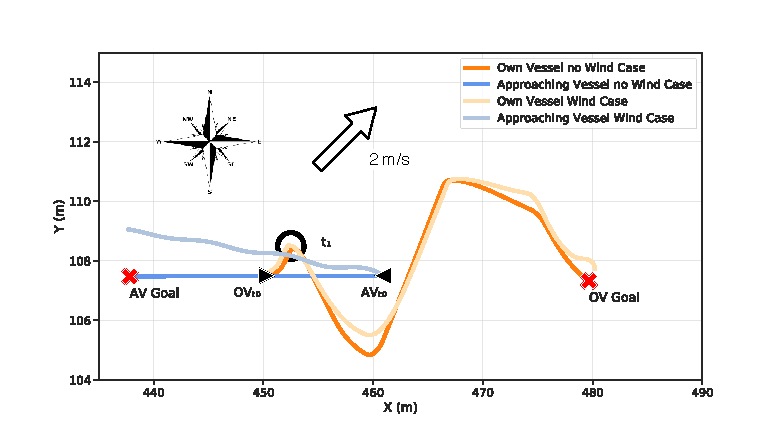
\includegraphics[width=\textwidth]{figs/Chap5/plot_ho_w_vs_wind.pdf}
            \caption{Comparison between the trajectories of the vessels in Wind case and no Wind case in a head-on encounter scenario, both cases use \ac{ATC} A*. Start position for \ac{OV} and \ac{AV} are marked with ">" and "<", while their goals are marked with "x". For the Wind case, the direction of the wind is northeast, represented by an arrow. We can observe that our \ac{ATC} A* kept implying COLREGS compliance even under the influence of wind in this scenario.}
            \label{fig:plot_ho_w_vs_wind}
        \end{figure}
        
        %%%%%%%%%%%%%%%%%%%%%%%%%%%%%%%%%%%%%%
        %% Head-On w vs wo Wind Computational Time
        %
        %% Grammarlly: 99/100
        %%%%%%%%%%%%%%%%%%%%%%%%%%%%%%%%%%%%%%
        Figure \ref{fig:plot_ho_w_vs_wind_CT} shows the computational time measured in seconds over time for wind and no wind cases. We observe that the computational time remains stable and does not seem to be related to the imposed wind influence for this simulation.
        \begin{figure}[H]
            \centering
            \includesvg[width=\textwidth]{figs/Chap5/plot_ho_w_vs_wind_CT.svg}
            \caption{Computational time comparison between Wind case versus no Wind in a head-on encounter.}
            \label{fig:plot_ho_w_vs_wind_CT}
        \end{figure}
        
        %%%%%%%%%%%%%%%%%%%%%%%%%%%%%%%%%%%%%%
        %% Crossing Right w vs wo \ac{ATC}. w vs wo Wind
        %
        %% Grammarlly: 100/100
        %%%%%%%%%%%%%%%%%%%%%%%%%%%%%%%%%%%%%%
        In Figure \ref{fig:plots_cr}, we present the behavior of our system when \ac{OV} encounters another vessel coming from the right side. In Figure \ref{fig:plot_cr_w_vs_wo}, we show the comparison between trajectories with and without ATC and in Figure \ref{fig:plot_cr_w_vs_wo_CT} we can see computational time for each case. As we can see, our method implies COLREGS compliance when avoiding a collision. In Figure \ref{fig:plot_cr_w_vs_wind} we show the comparison between trajectories with and without wind influence and in Figure \ref{fig:plot_cr_w_vs_wind_CT} we can see computational time for each case. Our method kept COLREGS-compliant even when disturbed by a maximum of 2.0 m/s wind.
        
        \begin{figure}[H]
        \centering
        
            \begin{subfigure}[b]{0.49\textwidth}
                \centering
                \includesvg[width=\textwidth]{figs/Chap5/plot_cr_w_vs_wo.svg}
                % \caption{Trajectory comparison between \ac{ATC} and no \ac{ATC} cases.}
                \caption{}
                \label{fig:plot_cr_w_vs_wo}
            \end{subfigure}
            \begin{subfigure}[b]{0.49\textwidth}
                \centering
                \includesvg[width=\textwidth]{figs/Chap5/plot_cr_w_vs_wo_CT.svg}
                % \caption{Computation Time. \ac{ATC} and no \ac{ATC} cases.}
                \caption{}
                \label{fig:plot_cr_w_vs_wo_CT}
            \end{subfigure}
            
            \begin{subfigure}[b]{0.49\textwidth}
                \centering
                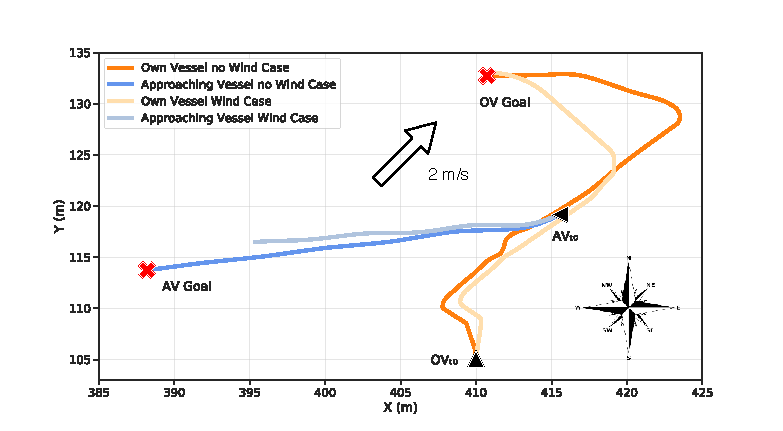
\includegraphics[width=\textwidth]{figs/Chap5/plot_cr_w_vs_wind.pdf}
                % \caption{Trajectory comparison between Wind and no Wind cases}
                \caption{}
                \label{fig:plot_cr_w_vs_wind}
            \end{subfigure}
            \begin{subfigure}[b]{0.49\textwidth}
                \centering
                \includesvg[width=\textwidth]{figs/Chap5/plot_cr_w_vs_wind_CT.svg}
                % \caption{Computation Time. Wind and no Wind cases.}
                \caption{}
                \label{fig:plot_cr_w_vs_wind_CT}
            \end{subfigure}
        
        \caption{Crossing Right Encounter Scenario. Comparison between \ac{ATC} and no \ac{ATC} (a and b), and Wind cases (c and d).}
        \label{fig:plots_cr}
        \end{figure}
        %AMA descobriu pq sem vento a curva mais mais longa do q com vento? parece estar invertido. convem verificar pois vao perguntar isso. nao esta fazendo  sentido.
        
         %AMA pq a posicao final do EV eh diferente com e sem vento ?
         
        In Figure \ref{fig:plot_cr_w_vs_wind}, in the time window we show, the \ac{AV} do not achieve its goal, the wind acts against \ac{AV} motion, reducing the maximum speed.
        %AMA nao entendi. quem nao atinge o objetivo ? na figura parece q sim. Ainda nao tem uma explicacao pq com vento a curva ficou melhor q sem vento
        
        %%%%%%%%%%%%%%%%%%%%%%%%%%%%%%%%%%%%%%
        %% Overtaking w vs wo \ac{ATC}. w vs wo Wind
        %
        %% Grammarlly: 100/100
        %%%%%%%%%%%%%%%%%%%%%%%%%%%%%%%%%%%%%%
        In Figure \ref{fig:plots_cl}, we present the behavior of our system in an overtaking encounter.
        %AMA ZOOOONA. o texto diz q eh overtaking e a legenda diz q eh crossin right. olhando a figura parece que a figura esta certa e o texto errado.mas esse tipo de erro da um no no leitor pois ele comeca a duvidar se entendeu alguma coisa.
        In Figure \ref{fig:plot_cl_w_vs_wo} we show the comparison between trajectories with and without \ac{ATC} and in Figure \ref{fig:plot_cl_w_vs_wo_CT} we can see computational time for each case. In an overtaking encounter, \ac{OV} must keep moving ahead, avoiding to generate any other crossing situations while overtaking. In our simulation, \ac{OV} avoids going to the front of \ac{AV} until it gets near the goal.
        In Figure \ref{fig:plot_cl_w_vs_wind} we show the comparison between trajectories with and without wind influence and in Figure \ref{fig:plot_cl_w_vs_wind_CT} we can see computational time for each case. Our method kept COLREGS-compliant even when disturbed by a maximum of 2.0 m/s wind.
        \begin{figure}[H]
        \centering
        
            \begin{subfigure}[b]{0.49\textwidth}
                \centering
                \includesvg[width=\textwidth]{figs/Chap5/plot_cl_w_vs_wo.svg}
                \caption{Trajectory}
                \label{fig:plot_cl_w_vs_wo}
            \end{subfigure}
            \begin{subfigure}[b]{0.49\textwidth}
                \centering
                \includesvg[width=\textwidth]{figs/Chap5/plot_cl_w_vs_wo_CT.svg}
                \caption{Computation Time}
                \label{fig:plot_cl_w_vs_wo_CT}
            \end{subfigure}
            
            \begin{subfigure}[b]{0.49\textwidth}
                \centering
                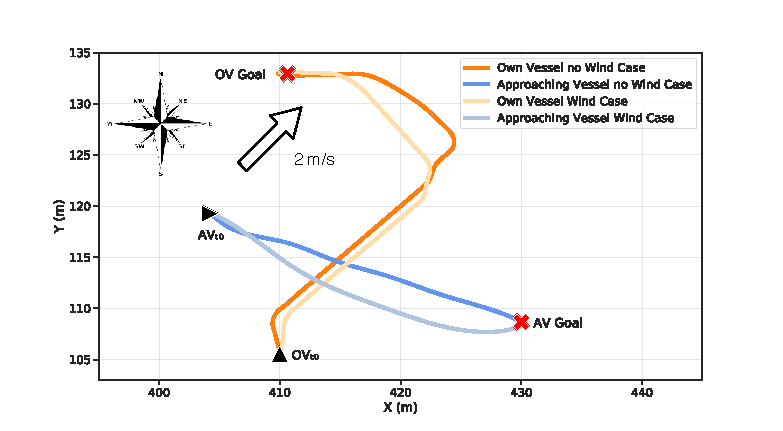
\includegraphics[width=\textwidth]{figs/Chap5/plot_cl_w_vs_wind.pdf}
                \caption{Trajectory}
                \label{fig:plot_cl_w_vs_wind}
            \end{subfigure}
            \begin{subfigure}[b]{0.49\textwidth}
                \centering
                \includesvg[width=\textwidth]{figs/Chap5/plot_cl_w_vs_wind_CT.svg}
                \caption{Computation Time}
                \label{fig:plot_cl_w_vs_wind_CT}
            \end{subfigure}
        
        \caption{Crossing Right Encounter Scenario. Comparing \ac{ATC} versus no \ac{ATC} cases and, with and Wind vs no Wind cases.}
        \label{fig:plots_cl}
        \end{figure}
        %AMA vc nao ia tentar refazer esse resltado p ver se sai essa barriga ?
        %AMA nao eh so para esse caso. esta faltando um paragrafro q discute o resultado. vc esta basicamente so largando as figuras sem nehuma discussao ou explicacao do reaultado obtido. cada caso deve ter uma discussao. nao eh o suficiente somente dizer se conseguiu ou nao realizar.
        %AMA pq tem uma diff no tempo de execucao com e sem vento ? FALTA DISCUSSAO !!!!
      
        
        %%%%%%%%%%%%%%%%%%%%%%%%%%%%%%%%%%%%%%
        %% Overtaking w vs wo \ac{ATC}. w vs wo Wind
        %
        %% Grammarlly: 100/100
        %%%%%%%%%%%%%%%%%%%%%%%%%%%%%%%%%%%%%%
        In Figure \ref{fig:plots_ov}, we present the behavior of our system when \ac{OV} encounters another vessel ahead.  %AMA a legenda diz overtaking ... confere os nomes e mantem a coerencia
        %AMA isso ainda nao foi corrigido !!!
        In Figure \ref{fig:plot_ov_w_vs_wo} we show the comparison between trajectories with and without ATC and in Figure \ref{fig:plot_ov_w_vs_wo} we can see computational time for each case. As we can see, once again, our method implies COLREGS compliance when avoiding a collision. In Figure \ref{fig:plot_ov_w_vs_wind} we show the comparison between trajectories with and without wind influence and in Figure \ref{fig:plot_ov_w_vs_wind_CT} we can see computational time for each case. 
        \begin{figure}[H]
        \centering
        
            \begin{subfigure}[b]{0.49\textwidth}
                \centering
                \includesvg[width=\textwidth]{figs/Chap5/plot_ov_w_vs_wo.svg}
                \caption{Trajectory}
                \label{fig:plot_ov_w_vs_wo}
            \end{subfigure}
            \begin{subfigure}[b]{0.49\textwidth}
                \centering
                \includesvg[width=\textwidth]{figs/Chap5/plot_ov_w_vs_wo_CT.svg}
                \caption{Computation Time}
                \label{fig:plot_ov_w_vs_wo_CT}
            \end{subfigure}
            
            \begin{subfigure}[b]{0.49\textwidth}
                \centering
                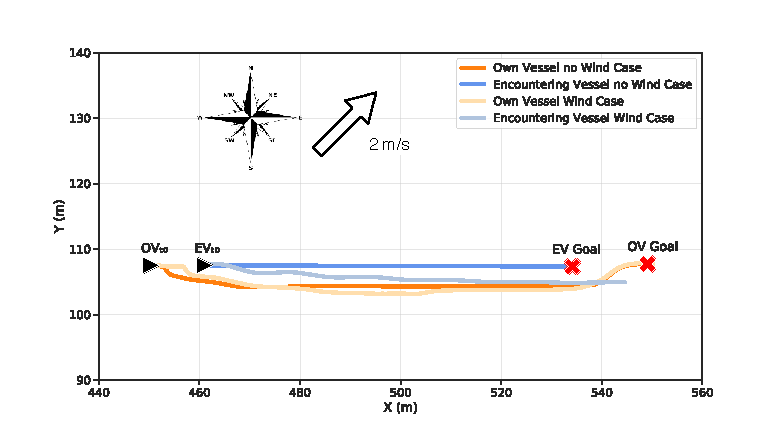
\includegraphics[width=\textwidth]{figs/Chap5/plot_ov_w_vs_wind.pdf}
                \caption{Trajectory}
                \label{fig:plot_ov_w_vs_wind}
            \end{subfigure}
            \begin{subfigure}[b]{0.49\textwidth}
                \centering
                \includesvg[width=\textwidth]{figs/Chap5/plot_ov_w_vs_wind_CT.svg}
                \caption{Computation Time}
                \label{fig:plot_ov_w_vs_wind_CT}
            \end{subfigure}
        
        %% Grammarlly: 100/100
        \caption{Overtaking Encounter Scenario with \ac{ATC}, with and without wind. In \ref{fig:plot_ov_w_vs_wind_CT} we can see a considerable increase in computation time from around 3 minutes until around 4min and 25 seconds. This happened due to the second limitation discovered in our method. With \ac{ATC}, the creation of virtual obstacles can be conflicting with the A* goal location and its neighbors. In this situation, the planner is not able to decide the route to be followed and decided to use the last generated speed command until the position of the A* goal location is free. Due to the conflicting position of the created virtual obstacle and local A* goal, the computational time cost achieves great value, since it explored the whole search space and found no solution.}
        \label{fig:plots_ov}
        \end{figure}
        %AMA acho melhor mover as dicussoes p o texto e nao deixar na legenda.
        
        %% Grammarlly: 100/100
        In Table \ref{tab:results}, we summarize the results for the different simulations we have done. In simulation scenarios, we can see that the computational time peak stays in a range from 0.355 to 0.390 for no \ac{ATC} configuration, from 0.357 to 0.395 for \ac{ATC} configuration and from 0.355 to 0.8852 for Wind configuration. Computation time for no \ac{ATC} and \ac{ATC} are similar since our \ac{ATC} method has a low impact on the A* implementation. With the influence of wind, we see an increase in the computational time peak. For the Overtaking scenario, the influence of wind led our system to an exhaustive scenario search in the whole search space. 
        %AMA algumas das discussoes q eu reclamei q faltavam estao aqui. Note que eu mencionei ALGUMAS .... 
        % mas vc deve lembrar q o leitor vai ler em ordem. Assim, ele vai ficar com duvidas ate chegar nesse ponto. Nesses casos, vc deve mencionar que, la onde a explicacao tinha q aparecer inicialmente, vc vai discutir tal coisa a seguir.
        
        %% Grammarlly: 96/100
        The average time stays similar for each scenario, regardless the configuration (no \ac{ATC}, \ac{ATC}, and Wind). In all cases presented, there is at least a 4.6 ratio between the maximum and average time. The high values reached occur when there is some considerable restriction in the search space, that is, when the goal for the local A* conflicts with the current position of \ac{AV} or with the created virtual obstacle. The average time remains low because the search in 100x100 search space does not demand much effort from the system, considering the platform where we perform the simulation and execution just needed to generate short and straight paths ahead. Regarding minimum distance, in our simulations, our system kept at least a safe distance of 1.505 meters from \ac{AV}. 
        %AMA e isso eh considerado safe ? de acordo c o que  ou quem ? importante discutir isso.
        %AMA note q na tabela em uma min distance de 0.7 m !!!
        
        
        %\ac{COLREGS} do not specify a specific value for safe distance or a proportion related to \ac{OV}'s size, but for some authors \cite{} \acp{USV} should at least keep a safe distance as the size of the vessel.
        % The average time keeps similar for each scenario encounter, not depending on the configuration (no \ac{ATC}, \ac{ATC}, and Wind) and consumed at least 4.6 times less time. 
        % Regarding minimum distance, in our simulations, our system kept at least a safe distance of 1.505 meters from \ac{AV}. %\ac{COLREGS} do not specify a specific value for safe distance or a proportion related to \ac{OV}'s size, but for some authors \cite{} \acp{USV} should at least keep a safe distance as the size of the vessel.

\begin{table}
\caption{Based on \cite{Lazarowska2017New, Singh2018Constrained, Agrawal2015COLREGS, Candeloro2017Voronoi, Svec2013Dynamics}, we made a quantitative evaluation of our planning system measuring computational cost and the minimum distance kept between the vessels during simulations.}
\label{tab:results}
\centering
\begin{tabular}{ccccccc} 
\toprule
\multirow{2}{*}{\begin{tabular}[c]{@{}c@{}}\textbf{Encounter}\\\textbf{Type} \end{tabular}}     & \multirow{2}{*}{\textbf{Case} } & \multicolumn{3}{c}{\textbf{Computational Time (s)} }          & \multirow{2}{*}{\begin{tabular}[c]{@{}c@{}}\textbf{Successful }\\\textbf{Avoidance }\end{tabular}} & \multirow{2}{*}{\begin{tabular}[c]{@{}c@{}}\textbf{Minimum }\\\textbf{Distance (m) }\end{tabular}}  \\ 
\cmidrule[\heavyrulewidth]{3-5}
                                                                                                &                                 & \textbf{Maximum} & \textbf{Average} & \textbf{Std. Variation} &                                                                                                    &                                                                                                     \\ 
\toprule
\multirow{3}{*}{\textbf{Head-On}}                                                               & \textbf{No ATC}                 & 0.369            & 0.136            & 0.061                   & Yes                                                                                                & 4.431                                                                                               \\
                                                                                                & \textbf{ATC}                    & 0.364            & 0.129            & 0.056                   & Yes                                                                                                & 1.599                                                                                               \\
                                                                                                & \textbf{Wind}                   & 0.355            & 0.131            & 0.060                   & Yes                                                                                                & 1.505                                                                                               \\ 
\cline{2-7}
\multirow{3}{*}{\begin{tabular}[c]{@{}c@{}}\textbf{Crossing}\\\textbf{from Right}\end{tabular}} & \textbf{No ATC}                 & 0.390            & 0.178            & 0.107                   & Yes                                                                                                & 5.414                                                                                               \\
                                                                                                & \textbf{ATC}                    & 0.390             & 0.249            & 0.060                   & Yes                                                                                                & 3.264                                                                                               \\
                                                                                                & \textbf{Wind}                   & 0.403            & 0.253            & 0.062                   & Yes                                                                                                & 3.739                                                                                               \\ 
\cline{2-7}
\multirow{3}{*}{\begin{tabular}[c]{@{}c@{}}\textbf{Crossing}\\\textbf{from Left}\end{tabular}}  & \textbf{No ATC}                 & 0.416                 & 0.235                 & 0.105                        &  Yes                                                                                                  & 7.018                                                                                                    \\
                                                                                                & \textbf{ATC}                    & 0.389                 & 0.224                 & 0.091                        & Yes                                                                                                   & 6.274                                                                                                    \\
                                                                                                & \textbf{Wind}                   & 0.400                 & 0.208                 & 0.102                        & Yes                                                                                                   & 5.707                                                                                                    \\ 
\cline{2-7}
\multirow{3}{*}{\textbf{Overtaking}}                                                            & \textbf{No ATC}                 & 0.368            & 0.006            & 0.030                   & Yes                                                                                                & 3.325                                                                                               \\
                                                                                                & \textbf{ATC}                    & 0.357            & 0.018            & 0.022                   & Yes                                                                                                & 3.101                                                                                               \\
                                                                                                & \textbf{Wind}                   & 0.852            & 0.039            & 0.073                   & Yes                                                                                                & 1.787                                                                                               \\
\bottomrule
\end{tabular}
\end{table}
%AMA discuta pq crossing from left tem tempos menores (max, avg, std var)
%AMA discuta p o maximo da ultima linha eh tao maior q os outros